%%
%% Automatically generated file from DocOnce source
%% (https://github.com/hplgit/doconce/)
%%
%%


%-------------------- begin preamble ----------------------

\documentclass[%
oneside,                 % oneside: electronic viewing, twoside: printing
final,                   % draft: marks overfull hboxes, figures with paths
10pt]{article}

\listfiles               %  print all files needed to compile this document
\usepackage{mathtools}
\usepackage{relsize,makeidx,color,setspace,amsmath,amsfonts,amssymb}
\usepackage[table]{xcolor}
\usepackage{bm,ltablex,microtype}
\usepackage{float}
\usepackage[pdftex]{graphicx}
\usepackage{epstopdf}
\usepackage{verbatim}

\usepackage{fancyvrb} % packages needed for verbatim environments

\usepackage[T1]{fontenc}
%\usepackage[latin1]{inputenc}
\usepackage{ucs}
\usepackage[utf8x]{inputenc}
\usepackage[english]{babel}
\usepackage{lmodern}         % Latin Modern fonts derived from Computer Modern

% Hyperlinks in PDF:
\definecolor{linkcolor}{rgb}{0,0,0.4}
\usepackage{hyperref}
\hypersetup{
    breaklinks=true,
    colorlinks=true,
    linkcolor=linkcolor,
    urlcolor=linkcolor,
    citecolor=black,
    filecolor=black,
    %filecolor=blue,
    pdfmenubar=true,
    pdftoolbar=true,
    bookmarksdepth=3   % Uncomment (and tweak) for PDF bookmarks with more levels than the TOC
    }
%\hyperbaseurl{}   % hyperlinks are relative to this root

\setcounter{tocdepth}{2}  % levels in table of contents



% prevent orhpans and widows
\clubpenalty = 10000
\widowpenalty = 10000

% --- end of standard preamble for documents ---


% insert custom LaTeX commands...

\raggedbottom
\makeindex
\usepackage[totoc]{idxlayout}   % for index in the toc
\usepackage[nottoc]{tocbibind}  % for references/bibliography in the toc

%-------------------- end preamble ----------------------

\begin{document}

% matching end for #ifdef PREAMBLE

\newcommand{\exercisesection}[1]{\subsection*{#1}}


% ------------------- main content ----------------------



% ----------------- title -------------------------

\thispagestyle{empty}

\begin{center}
{\LARGE\bf
\begin{spacing}{1.25}
PHYS 905 - Project 2
\end{spacing}
}
\end{center}

% ----------------- author(s) -------------------------

\begin{center}
{\bf Terri Poxon-Pearson}
\end{center}

    
% ----------------- end author(s) -------------------------

% --- begin date ---
\begin{center}
February 27, 2017
\end{center}
% --- end date ---

\vspace{1cm}

INSERT ABSTRACT HERE

\tableofcontents
 
\section{Introduction}
In this project we will be solving Schroedinger's equation for the case of electrons in a 3D harmonic oscillator. First, we will first solve the simpler, non-interacting case with just one electron in the harmonic oscillator potential using Jacobi's method. Next, we will add a second electron with interacts via a repulsive, Coulomb potential.  This will involve a change into center of mass coordinates.  Both problems will be solved for l=0 case.  Additionally, we will explore our calculation's sensitivity to parameters such as the number of mesh points and maximum integration radius.

This report will begin with a brief introduction to the physical system we are studying in this project, as well as a description of how these equations are discretized.  Next I will describe the method used to solve this eigenvalue problem.  I will discuss the implementation of this algorithm, including a discussion of sensitivity to various integration variables and tests used to check the code's validity.  Finally, I will present the results of my calculations, followed by some conclusions and perspectives for future calculations.

\section{Methods}

\subsection{Physics of Single Electron in 3D Oscillator}

If we assume spherical symmetry, the radial part of Shroedinger's equation for a single electron in a harmonic oscillator can be writen as

\begin{equation*}
  -\frac{\hbar^2}{2 m} \left ( \frac{1}{r^2} \frac{d}{dr} r^2
  \frac{d}{dr} - \frac{l (l + 1)}{r^2} \right )R(r) 
     + V(r) R(r) = E R(r).
\end{equation*}

where $V(r)$ is the harmonic oscillator potential.  The energies $E$ for the 3D harmonic oscilator are well know and given by

\begin{equation*}
E_{nl}=  \hbar \omega \left(2n+l+\frac{3}{2}\right).
\end{equation*}

To simplify the expression, we can make the common substitution $R(r) = (1/r) u(r)$, leaving us with
% 

\begin{equation*}
  -\frac{\hbar^2}{2 m} \frac{d^2}{dr^2} u(r) 
       + \left ( V(r) + \frac{l (l + 1)}{r^2}\frac{\hbar^2}{2 m}
                                    \right ) u(r)  = E u(r) .
\end{equation*}
% 

We have two boundary conditions to constrain this differential equations.  First, we want the wave function to disappear at the origin, so $u(0)=0$.  Second, the wave function should be localized to the oscillator well, so we want $u(\infty)=0$.  Here, we will only consider $l=0$ states, which eliminates one term of the equation.  Finally, we can indroduce a dimensionless variable $\rho = (1/\alpha) r$ and insert  $V(\rho) = (1/2) k \alpha^2\rho^2$, leaving us with

\begin{equation*}
  -\frac{\hbar^2}{2 m \alpha^2} \frac{d^2}{d\rho^2} u(\rho) 
       + \frac{k}{2} \alpha^2\rho^2u(\rho)  = E u(\rho) .
\end{equation*}

Multiplying through my the leading factors leaves us with

\begin{equation*}
  -\frac{d^2}{d\rho^2} u(\rho) 
       + \frac{mk}{\hbar^2} \alpha^4\rho^2u(\rho)  = \frac{2m\alpha^2}{\hbar^2}E u(\rho) .
\end{equation*}

Now we can choose that

\begin{equation*}
\frac{mk}{\hbar^2} \alpha^4 = 1
\end{equation*}

and define

\begin{equation*}
\lambda = \frac{2m\alpha^2}{\hbar^2}E.
\end{equation*}

That leaves us with the final expression

\begin{equation*}
  -\frac{d^2}{d\rho^2} u(\rho) + \rho^2u(\rho)  = \lambda u(\rho) .
\end{equation*}

This is the equation that we must solve numerically.  There are analytic solutions in the case of $l=0$ and the three lowest eigen values are $\lambda_0=3,\lambda_1=7,\lambda_2=11$. We can compare the accuracy of our results to these exact solutions.

\subsection{Discretization of Schroedinger's Equation}

As in Project 1, we will discretize the differential equation and use the three point formula to express the second derivative.  This expression is given by
 
\begin{equation*}
    u''=\frac{u(\rho+h) -2u(\rho) +u(\rho-h)}{h^2} +O(h^2).
    \label{eq:diffoperation}
\end{equation*}

A full derivation of this expression can be found in \cite{LectureNotes}.  Here, $h$ is the step size where 

\begin{equation*}
  h=\frac{\rho_N-\rho_0 }{N}
\end{equation*}

and the value of $\rho$ at a point $i$ is then 

\[
    \rho_i= \rho_0 + ih \hspace{1cm} i=1,2,\dots , N.
\]

$N$ defines the number of grid points. Because this is a radial integral, the define minimum value for $\rho$ is 0 and  $\rho_{\mathrm{max}}=\rho_N$,

Using the compact notation from project one, we can rewrite the Schroedinger equation as

\[
-\frac{u_{i+1} -2u_i +u_{i-1}}{h^2}+\rho_i^2u_i=-\frac{u_{i+1} -2u_i +u_{i-1} }{h^2}+V_iu_i  = \lambda u_i,
\]
where $V_i=\rho_i^2$ is the harmonic oscillator potential.

This expression can also be cast as a matrix equation.  The left hand side takes the form of a modified tridiagonal matrix.  Instead of just having 2 in the diagonal and -1 in the off diagonal, non-zero elements, we now have 

\begin{equation*}
   d_i=\frac{2}{h^2}+V_i
\end{equation*}
and 
\begin{equation*}
   e_i=-\frac{1}{h^2}.
\end{equation*}

Instead of having some known function $f$ on the right hand side, we instead have $\lambda \cdot u$.  Now, for each point on the wavefuntion $u_i$, we can define the Schroedinger equation takes the following form

\begin{equation*}
d_iu_i+e_{i-1}u_{i-1}+e_{i+1}u_{i+1}  = \lambda u_i,
\end{equation*}

This is, of course, the form of an eigenvalue problem and the entire matrix can be written as
\begin{equation}
 \begin{bmatrix} \frac{2}{h^2}+V_1 & -\frac{1}{h^2} & 0   & 0    & \dots  &0     & 0 \\
                                -\frac{1}{h^2} & \frac{2}{h^2}+V_2 & -\frac{1}{h^2} & 0    & \dots  &0     &0 \\
                                0   & -\frac{1}{h^2} & \frac{2}{h^2}+V_3 & -\frac{1}{h^2}  &0       &\dots & 0\\
                                \dots  & \dots & \dots & \dots  &\dots      &\dots & \dots\\
                                0   & \dots & \dots & \dots  &-\frac{1}{h^2}  &\frac{2}{h^2}+V_{N-2} & -\frac{1}{h^2}\\
                                0   & \dots & \dots & \dots  &\dots       &-\frac{1}{h^2} & \frac{2}{h^2}+V_{N-1}
             \end{bmatrix}  \begin{bmatrix} u_{0} \\
                                                              u_{1} \\
                                                              \dots\\ \dots\\ \dots\\
                                                              u_{N}
             \end{bmatrix}=\lambda \begin{bmatrix} u_{0} \\
                                                              u_{1} \\
                                                              \dots\\ \dots\\ \dots\\
                                                              u_{N}
             \end{bmatrix}.  
      \label{eq:sematrix}
\end{equation}
Since the values of $u$ at the two endpoints are known via the boundary conditions, we can skip the rows and columns that involve these values.

\subsection{Jacobi's Rotation Algorithm}

In this project we implement Jacobi's method to solve the eigenvalue problem.  I will briefly explain the method here, but a full explanation of the method can be found in \cite{LectureNotes}.  The method is based on a series of rotations performed on the matrix which eliminates the off diagonal matrix elements.  These rotations are allowable because unitary transformations preserve orthogonality.  For a proof of this property, see \ref{A}.

Because we want to eliminate off diagonal elements of the array, we search the matrix for the largest off-diagonal element.  Once I identified, we need to determine the rotation angle that will bring this element to 0.  For the identified largest element, $a_{kl}$, we can find this angle through the relation

\begin{equation*}
\cot 2\theta=\tau = \frac{a_{ll}-a_{kk}}{2a_{kl}}.
\end{equation*}

We can then define the angle $\theta$ by using the relation $\cot 2\theta=1/2(\cot \theta-\tan\theta)$.  Solving for $tan(\theta)$ $(t)$ we get

\begin{equation*}
  t = -\tau \pm \sqrt{1+\tau^2}.
\end{equation*}

Finally, $t$ can be easily related to $cos(\theta) (c)$ and $sin(\theta) (s)$ by

\begin{equation*}
   c = \frac{1}{\sqrt{1+t^2}}
\end{equation*}

and

\begin{equation*} 
s=tc
\end{equation*}

Once the rotation angle is determined, we apply the transformation.  After the transformation, the matrix elements are changed so that

\begin{equation*}
\begin{split}
& b_{ii}=a_{ii} (i \ne k, j \ne l) \\
& b_{ik}=a_{ik}c - a_{il}s  (i \ne k, j \ne l) \\
& b_{il}=a_{il}c + a_{ik}s  (i \ne k, j \ne l) \\
& b_{kk}=a_{kk}c^2 -2a_{kl}cs + a_{ll}s^2 \\
& b_{kk}=a_{ll}c^2 +2a_{kl}cs + a_{kk}s^2 \\
& b_{kl} = 0.
\end{split}
\end{equation*}

This process can then be repeated until all off diagonal elements are effectively 0 (less than some defined tolerance).  When the process is complete, you will have a diagonal matrix with eigenvalues along the diagonal.  Finally, the corresponding eigenvectors are easy to obtain.  Originally, we define an NXN unit matrix, $r$, which is the same size as the matrix being diagonalized.  Then, after each transformation, this matrix can be transformed using the relation

\begin{equation*}
\begin{split}
&r_{ik} = r_{ik}c-r_{il}s \\
&r_{il} = r_{il}c + r_{ik}s.
\end{split}
\end{equation*}

\subsection{Physics of Interacting Electrons in 3D Oscillator}

If we now add a second electron to the harmonic oscillator, they will interact through the Coulomb force.  If there was no interaction, we would just have the sum of two single particle Schroedinger equations, which can be written as 

\begin{equation*}
\left(  -\frac{\hbar^2}{2 m} \frac{d^2}{dr_1^2} -\frac{\hbar^2}{2 m} \frac{d^2}{dr_2^2}+ \frac{1}{2}k r_1^2+ \frac{1}{2}k r_2^2\right)u(r_1,r_2)  = E^{(2)} u(r_1,r_2) 
\end{equation*}


where $u(r_1,r_2)$ is a two electron wave function and $E^{(2)}$ is the two electron energy.

To simplify this problem, we can perform a change of variables.  We will use the relative coordinate $\mathbf{r} = \mathbf{r}_1-\mathbf{r}_2$
and the center-of-mass coordinate $\mathbf{R} = 1/2(\mathbf{r}_1+\mathbf{r}_2)$.  This gives us

\begin{equation*}
\left(  -\frac{\hbar^2}{m} \frac{d^2}{dr^2} -\frac{\hbar^2}{4 m} \frac{d^2}{dR^2}+ \frac{1}{4} k r^2+  kR^2\right)u(r,R)  = E^{(2)} u(r,R).
\end{equation*}

As shown in \cite{Broida}, the equations for $r$ and $R$ can be separated via the ansatz for the 
wave function $u(r,R) = \psi(r)\phi(R)$ and the energy is given by

\begin{equation*}
E^{(2)}=E_r+E_R.
\end{equation*}

Now if we add the Coulomb term,

\begin{equation*}
V(r_1,r_2) =\frac{\beta e^2}{r},
\end{equation*}
with $\beta e^2=1.44$ eVnm, we get

\begin{equation*}
\left(  -\frac{\hbar^2}{m} \frac{d^2}{dr^2}+ \frac{1}{4}k r^2+\frac{\beta e^2}{r}\right)\psi(r)  = E_r \psi(r).
\end{equation*}

If we preform a similar process of multiplying through by leading coefficients and reintroduce the dimensionless variable $\rho = r/\alpha$, we get
\begin{equation*}
  -\frac{d^2}{d\rho^2} \psi(\rho) 
       + \frac{1}{4}\frac{mk}{\hbar^2} \alpha^4\rho^2\psi(\rho)+\frac{m\alpha \beta e^2}{\rho\hbar^2}\psi(\rho)  = 
\frac{m\alpha^2}{\hbar^2}E_r \psi(\rho) .
\end{equation*}

Now wi will massage this equation to create an analogue to the non-interacting case.  To do this, we define a new 'frequency'

\begin{equation*}
\omega_r^2=\frac{1}{4}\frac{mk}{\hbar^2} \alpha^4,
\end{equation*}
and fix $\alpha$ by 
\begin{equation*}
\frac{m\alpha \beta e^2}{\hbar^2}=1
\end{equation*}

and define

\begin{equation*}
\lambda = \frac{m\alpha^2}{\hbar^2}E.
\end{equation*}

Now, we can rewrite Schroedinger's equation as

\begin{equation*}
  -\frac{d^2}{d\rho^2} \psi(\rho) + \omega_r^2\rho^2\psi(\rho) +\frac{1}{\rho} = \lambda \psi(\rho).
\end{equation*}

In this form, $\omega_r$ reflects the strength of the oscillator potential.

Here we studied the cases $\omega_r = 0.01$, $\omega_r = 0.5$, $\omega_r =1$,
and $\omega_r = 5$ for the ground state. Again, we only study $l=0$ states and we omit the center-of-mass energy.

\section{Code and Implementation}

All of the programs, results, and benchmarks for this work can be found in my GIT repository ( https://github.com/poxonpea/PHYS905 ).  All codes for this project were written in FORTRAN.

\subsection{Implementing Single and Interacting Electron Cases}

The code containing the heart of the Jacobi algorithm is shown below

\begin{figure}[H]\label{fig:Jacobi}
  \centering
    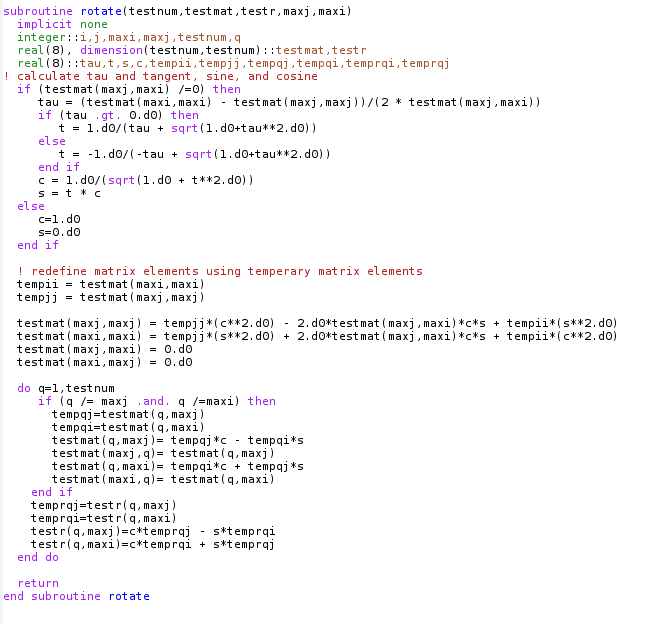
\includegraphics[width=1.2\textwidth]{Rotate.PNG}
    \caption{Code from Jacobi.f90 which implements Jacobi's Algorithm}
\end{figure}

This subroutine is implementing after a separate subroutine searches the matrix to find the largest off diagonal element.  When running Jacobi.f90, the user decides whether to run for 1 or 2 electrons.  The only difference is the potential used.  That can be seen in the code below.

\begin{figure}[H]\label{fig:Potential}
  \centering
    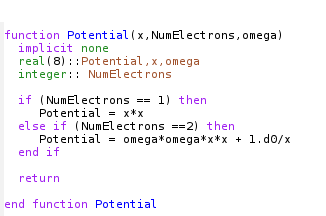
\includegraphics[width=0.8\textwidth]{Potential.PNG}
    \caption{The potential implemented in Jacobi.f90}
\end{figure}

Depending on the user choice, the code will either select the simpler, one electron potential, or the potential for the interacting case.

\subsection{Tests of Code}


\section{Results and Discussion}


\subsection{Exploring Dependence of Integration Parameters}

The results of the calculation will be sensitive to the choice of $\rho_{max}$ and $N$.  Both of these parameters can be defined by the user while running the program.  I explored the sensitivity to these parameters for the case of the non-interacting electron.  In three dimension, we know the eigenvalues for the three lowest lying, $l=0$ states should be $\lambda_0=3$, $\lambda_1=7$, and $\lambda_2=11$.  Below is a table of convergence for these results for different choices of  $\rho_{max}$ and $N$.

As you can see from the results, $\rho_{max}=6$ and $N=200$ is sufficient for convergence and I used this combination for my runs.

\subsection{Convergence}

\begin{figure}[H]\label{fig:3}
  \centering
    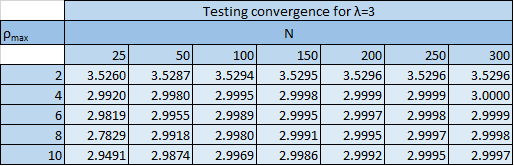
\includegraphics[width=1.1\textwidth]{3.png}
\end{figure}

\begin{figure}[H]\label{fig:7}
  \centering
    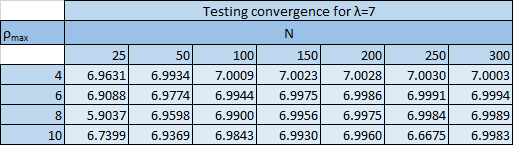
\includegraphics[width=1.1\textwidth]{7.png}
\end{figure}

\begin{figure}[H]\label{fig:11}
  \centering
    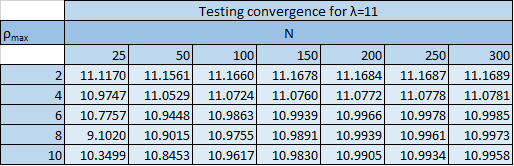
\includegraphics[width=1.1\textwidth]{11.png}
\end{figure}
\subsection{Computational Speeds}


\section{Conclusions}



\section{Appendices}

\subsection{Appendix A} \label{A}

Consider a basis of orthogonal basis vectors $\mathbf{v}_i$,
\[
\mathbf{v}_i = \begin{bmatrix} v_{i1} \\ \dots \\ \dots \\v_{in} \end{bmatrix}
\]

Orthogonality requires that 

\[
\mathbf{v}_j^T\mathbf{v}_i = \delta_{ij}.
\]

We can apply an orthogonal or unitary transformation such that

\[
\mathbf{w}_i=\mathbf{U}\mathbf{v}_i.
\]

Unitarity enforces that the product of a matrix with its conjugate transpose is the identity matrix.  Orthogonal matrices are a subset of real, unitary matrices.  This condition implies that the product of a matrix with its transpose is the identity matrix.  These two conditions can be expressed as

\[
\mathbf{U}^* \mathbf{U} = \mathbf{U} \mathbf{U}^* = \mathbb{I}
\]

\[
\mathbf{U}^T \mathbf{U} = \mathbf{U} \mathbf{U}^T = \mathbb{I}.
\]

If we now look at the product of our transformed matrix with its transpose, we find

\[
\mathbf{w}^T_j\mathbf{w}_i = (\mathbf{U}\mathbf{v}_i)^T(\mathbf{U}\mathbf{v}_j)= \mathbf{v}_i^T\mathbf{U}^T\mathbf{U}\mathbf{v}_j=\mathbf{v}_i^T\mathbf{U}\mathbf{U}^T\mathbf{v}_j =\mathbf{v}_j^T\mathbf{v}_i = \delta_{ij}.
\]

Therefore, the dot product is preserved.

\begin{comment}

\begin{figure}[H]\label{fig:compzoom}
  \centering
    \includegraphics[width=1.2\textwidth]{compzoom.eps}
    \caption{A zoomed in view of the convergence to the exact solution}
\end{figure}

\begin{center} 
\begin{tabular}{ |c|c|c|c| }
\hline
Size of Matrix ($10^n$) & General & Tailored & LU \\
\hline
1& 3.00 E -6 & 3.00 E -6 & 2.40 E -5\\ 
2 & 4.00 E -6 & 4.00 E -6 & 1.71 E -3 \\ 
3 & 3.90 E -5 & 1.90 E -5 & 1.93\\ 
4 & 3.79 E -4 & 2.09 E -4 & N/A\\ 
5 & 3.38 E -3 & 1.51 E -3  & N/A\\ 
6 & 2.87 E -2 & 1.53 E -2 & N/A\\ 
7 & 3.16 E -1 & 1.73 E -1& N/A\\ 
\hline
\end{tabular}
\label{table:test}
\end{center}

\end{comment}

\begin{thebibliography}{9}

\bibitem{LectureNotes} 
Hjorth-Jensen, Mortehn. 
Computational Physics, Lecture Notes Fall 2015. 
August 2015.


\bibitem{Broida}
Broida, J.
PHYS 130B, Quantum Mechanics II Class Notes.
Fall 2009.
http://www.physics.ucsd.edu/students/courses/fall2009/physics130b/IdentParts.pdf

\bibitem{ClassNotes} 
Hjorth-Jensen, Mortehn. 
Introduction to Programming. 
Computational Physics.
https://compphysics.github.io/ComputationalPhysicsMSU/doc/pub/languages/pdf/languages-minted.pdf.

\end{thebibliography}



% ------------------- end of main content ---------------

\end{document}

